% =====================================================================
%  Chapter 5 — \idxw{2024 YR4}: The Case Where the Response Failed
% =====================================================================

\chapter{2024 YR4: The Case Where the Response Failed}
\label{ch:yr4}

One object has been studied hard enough to expose every part of the problem
this book describes. It was discovered on the night of a close approach, it
was sized three different ways that disagree by a factor of 1.7 in diameter,
it is due to hit the Moon in 2032, and it has a formal warning attached to it
that is generated by a scale whose energy axis rests on those disagreeing
sizes.

The record is unusually complete, and it is worth reading closely because
almost every number in this book was checked against it.

\section{How it was found}

The JPL Small-Body Database records the first observation of 2024~YR4 on
25 December 2024. The close-approach record for the same date gives the
distance: 0.00554 astronomical units, or 828,775 kilometres, at a relative
velocity of 13.75 kilometres per second.

So the object was discovered on the very night it passed inside the Earth's
sphere of influence, at a distance of roughly five and a half lunar
distances. That is a discovery with almost no warning attached, and it is
worth noting that it was nonetheless a success: the object was found at
all, and its orbit was good enough that the 2032 lunar encounter could be
computed at all.

The orbit solution is not marginal. It uses 485 observations with a residual
of 0.45 arcseconds, and the absolute magnitude it carries is
\(23.93 \pm 0.28\). That last figure is worth holding on to, because the
2025 \idxw{JWST} analysis of the object gives \(24.14 \pm 0.25\), which is a
discrepancy of 0.21 magnitudes --- inside both uncertainties, and therefore
the sort of difference that ought not to change anything. It is carried
through this book rather than reconciled, because a reader checking the
catalogue against the literature should be able to see that the two agree as
well as they do.

\section{Three sizes, one object}

The 26 March 2025 JWST\idx{JWST} MIRI analysis is the most thorough physical
characterisation of any object of this class, and it is a study in the
degeneracy the earlier chapters described. The measurements it reports are
the following: a spin pole at galactic coordinates \((l, b) = (232^\circ,
-11^\circ)\); a sidereal rotation period of 19.4633 minutes; axis ratios
\(a/b \approx 1.28\) and \(b/c \approx 1.45\); an equivalent-volume diameter
of 60.8 metres with an uncertainty of \(+1.8\) and \(-3.6\) metres; a
geometric albedo of \(0.11^{+0.05}_{-0.03}\) from the absolute magnitude
\(H_V = 24.14 \pm 0.25\); and a high thermal inertia with low surface
roughness.

Those are excellent numbers. The difficulty is that the object has not been
measured, and the size comes from a thermal model whose assumptions are
being fitted rather than tested.

\begin{table}[!htbp]
\centering
\small
\caption{The three thermal models in the published analysis of 2024 YR4, and
what each gives for the diameter.}
\label{tab:yr4-models}
\begin{tabularx}{\textwidth}{@{}P{1.65in}P{0.91in}Y@{}}
\toprule
\rowcolor{panel}
\textbf{Model} & \textbf{Diameter} & \textbf{Note} \\
\midrule
NEATM, standard & 60.6 m & requires a beaming parameter\idx{Beaming parameter} of 3.06, which is
unphysical, and is rejected \\
\rowcolor{panel}
Fast rotating model & 51.1 m & albedo 0.16 \\
\idxw{Thermophysical model} & 60.8 m & the published best fit \\
\bottomrule
\end{tabularx}
\end{table}

The two credible models differ by 19 per cent in diameter. Because volume
goes as the cube, that is a factor of 1.68 in energy at fixed density. The
object's physical description is therefore uncertain at the 20 per cent level
for a reason that has nothing to do with the quality of the observations and
everything to do with the choice of model.

\section{What that does to the hazard class}

Carried through \eqref{eq:energy} at the published lunar-impact speed of
14.1 kilometres per second and across the density range from a rubble pile
at 1,300 to a coherent body at 3,500 kilogrammes per cubic metre, the
published model set spans 2.16 to 9.79 megatons --- a factor of 4.5.

The decomposition is exact and it is the most useful single calculation in
this chapter. The thermal-model choice alone contributes a factor of
\((60.8/51.1)^3 = 1.68\), and the density choice alone contributes
\(3500/1300 = 2.69\). Their product is 4.53, against the published spread of
4.53. Two thirds of the uncertainty in the energy is a modelling choice; one
third is a composition assumption. Neither is an observational error.

\begin{figure}[!htbp]
\centering
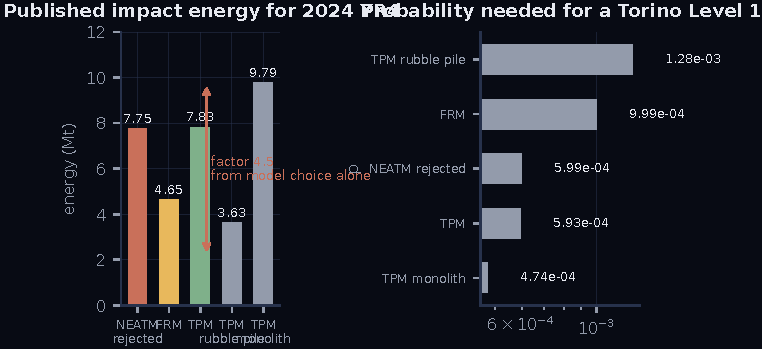
\includegraphics[width=\textwidth]{../figures/fig_yr4.pdf}
\caption{Left: the impact energy of 2024 YR4 under the published model set.
Right: the probability required for a Torino Level 1, which moves with the
energy. The astrometry is identical in every case.}
\label{fig:yr4}
\end{figure}

Now apply \eqref{eq:level1}. The Level 1 threshold probability for this object
is \(4.64\times 10^{-3}/E\), so the threshold ranges from \(4.7\times 10^{-4}\)
at 9.79 megatons to \(2.2\times 10^{-3}\) at 2.16 megatons. An object whose
orbit has not moved by a milliarcsecond can be Level 0 or Level 1 on the
strength of a modelling decision.

That is the accountability gap expressed as a single number, and it is why
the book's endpoint is accountability rather than detection.

\section{The encounter, and what it would have measured}

The object's next close approach is on 22 December 2032, at 0.00186
astronomical units or 278,333 kilometres from the Earth's centre. That
approach ends in an impact on the Moon, and the published accounts of it
disagree in a way that must be carried rather than reconciled: the JWST\idx{JWST}
analysis reports a lunar passage within \(22,900 \pm 800\) kilometres, while
the independent Monte Carlo study reports a nominal selenocentric closest
approach of 3,000 kilometres with a lunar B-plane uncertainty of 25,000
kilometres and 426 of 10,000 clones striking the Moon, giving 4.26 per cent;
the ejecta analysis uses 4 per cent. The difference is between a
closest-approach statistic weighted over the impact-probability distribution
and the nominal trajectory of a specific solution.

What matters for this book is what the geometry would allow a measurement to
do. At 22,900 kilometres a 60.8-metre object subtends 548 milliarcseconds,
which a 0.35-metre aperture resolves and a matched interferometric baseline
of 1.13 metres images with four samples across the diameter. At the
nominal 3,000-kilometre distance it subtends 4.18 arcseconds and the matched
baseline is 0.15 metres. In both cases the range is not inferred from an
orbit at all: the Moon's own ephemeris gives it directly, to the centimetre.

\section{The 2028 apparition, and the limit of the argument}

Between the 2024 discovery and the 2032 encounter, the object's only
opportunity is the 2028 apparition, an Earth encounter at 0.05 astronomical
units, where it is about 17.4 magnitudes and 1.68 milliarcseconds across.

This is where the book's argument must be careful, because a reader is
entitled to know what the lunar platform would and would not have bought.
The 2025 to 2028 interval was a \emph{distance} problem: the object was too
far from the Earth for any observatory to do useful work on it, and no
vantage point fixes that. And at 0.05 astronomical units the object is
unresolved and 1.68 milliarcseconds across, so a lunar station would have
measured its position, not its shape.

What the 2032 encounter offers is different and better: a resolved image at
short range, and a range that is known rather than fitted. The prediction the
book makes is therefore modest and falsifiable. With a lunar surface array,
the 2032 apparition would yield a resolved shape and a pole for 2024~YR4
from a range of 3,000 to 23,000 kilometres, and the shape would supply the
volume that the three thermal models cannot agree on. Without one, the shape
of 2024~YR4 will continue to be inferred from a convex lightcurve inversion
and a single thermal campaign, and the energy will remain uncertain by a
factor of about two.

\begin{keytakeaways}
\item 2024 YR4\idx{2024 YR4} was discovered on the night it passed at 828,775 kilometres,
and its 2032 encounter ends in an impact on the Moon.
\item Two credible thermal models differ by 19 per cent in diameter, which is
a factor of 1.68 in energy and nothing to do with the observations.
\item The energy spread of 4.5 decomposes exactly into 1.68 from the thermal
model and 2.69 from the density.
\item The Level 1 probability threshold moves from \(4.7\times10^{-4}\) to
\(2.2\times10^{-3}\) across that spread, with the astrometry untouched.
\end{keytakeaways}
